
\newpage

\subsection{The MSCI}
\label{subsection: MSCI Index}
The MSCI World Index captures large and mid cap representation across 23 Developmed Markets (DM) countries. As such, the difference compared to the well-known MSCI ACWI Index is the exclusive weight on assets from developed economies. With 1,600 constituents, the index covers approximately 85\% of the free-float-adjusted market captilization in each country. The weights across country and sectors are shown in figure XXXXY as of November 2020. The historical development of the index is depicted in figure \ref{fig:MSCI_index}. 
 
\begin{figure}[H] 
    \centering
    
\includegraphics[width=1.0\textwidth]{analysis/data_description/images/MSCI_index.png}
    \caption{Development MSCI.}
    \label{fig:MSCI_index}
\end{figure}

%##### INDSÆT FIGUR AF Sector og region focus ####### # VIS split

The inclusion of the MSCI World Index is based on the fact that it is a global index, and thus should capture the economics trends across geographies. As such, the thesis treats it as a baseline index in terms of uncovering economic-regimes. Although it is a world index, North America makes up almost 2/3 of the index, however, this makes sense from an economic perspective since the U.S. economy serves as a fundamental indicator of how the remaining world economy is progressing. Furthermore, the information technology sector is by far the largest sector in the index, since it accounts for approximately 22\% of the overall allocation as per figure XXXXX. It should be noted that the weights are a snapshot in time, hence they are constantly changing. 

\begin{table}[H]
\caption{Summary statistics for the daily MSCI log-returns.}
\centering
\begin{tabular}{c c c c c c c c c} 
\hline\hline
Observations & Mean & STD & Skewness & Excess Kurtosis & Min & Max & First ACF & Annual SR \\
\hline
12,941 & 0.0003 & 0.0087 & -0.6521 & 10.8819 & -0.1044 & 0.0909 & 0.1337 & 0.4854 \\
\hline
\end{tabular}
\label{tab:summary_stats_MSCI}
\end{table}

Table \ref{tab:summary_stats_MSCI} shows the first four central moments together with the minimum and maximum observation, the first-order autocorrelation and the annual Sharpe ratio (SR). The SR is the excess return per unit risk, i.e. the excess return divided by the standard deviation (SD). The first observations originates from 1969-12-31 and the final included observations is the date 2021-02-12. It appears that the daily log-returns for the MSCI World Index are negatively skewed and the distribution is also characterised by being highly leptokurtic as the excess kurtosis is positive. As such, the summary statistics indicate that the log return series for the MSCI World Index, are characterised by the set of stylized facts that are commonly associated with financial returns. The range of the observations has a span of 0.1953, thereby indicating that the index can change significantly in high-volatility periods.

\subsection{DAX 30}
\label{subsection: DAX 30}
The DAX is a blue chip stock market index comprising the 30 largest listed German companies. It is similar in nature to FTSE 100 and the Dow Jones Industrial Average. The index is included in the analysis in order to get an estimate for, whether the model parameters will change significantly when trained on the DAX as opposed to the aforementioned indexes. As such, the DAX becomes particularly interesting since its composition of a small number of firms and a restrictive geographical focus on Germany means that it might not necessarily represent the vitality of the economy as a whole. 

\begin{figure}[H] 
    \centering
    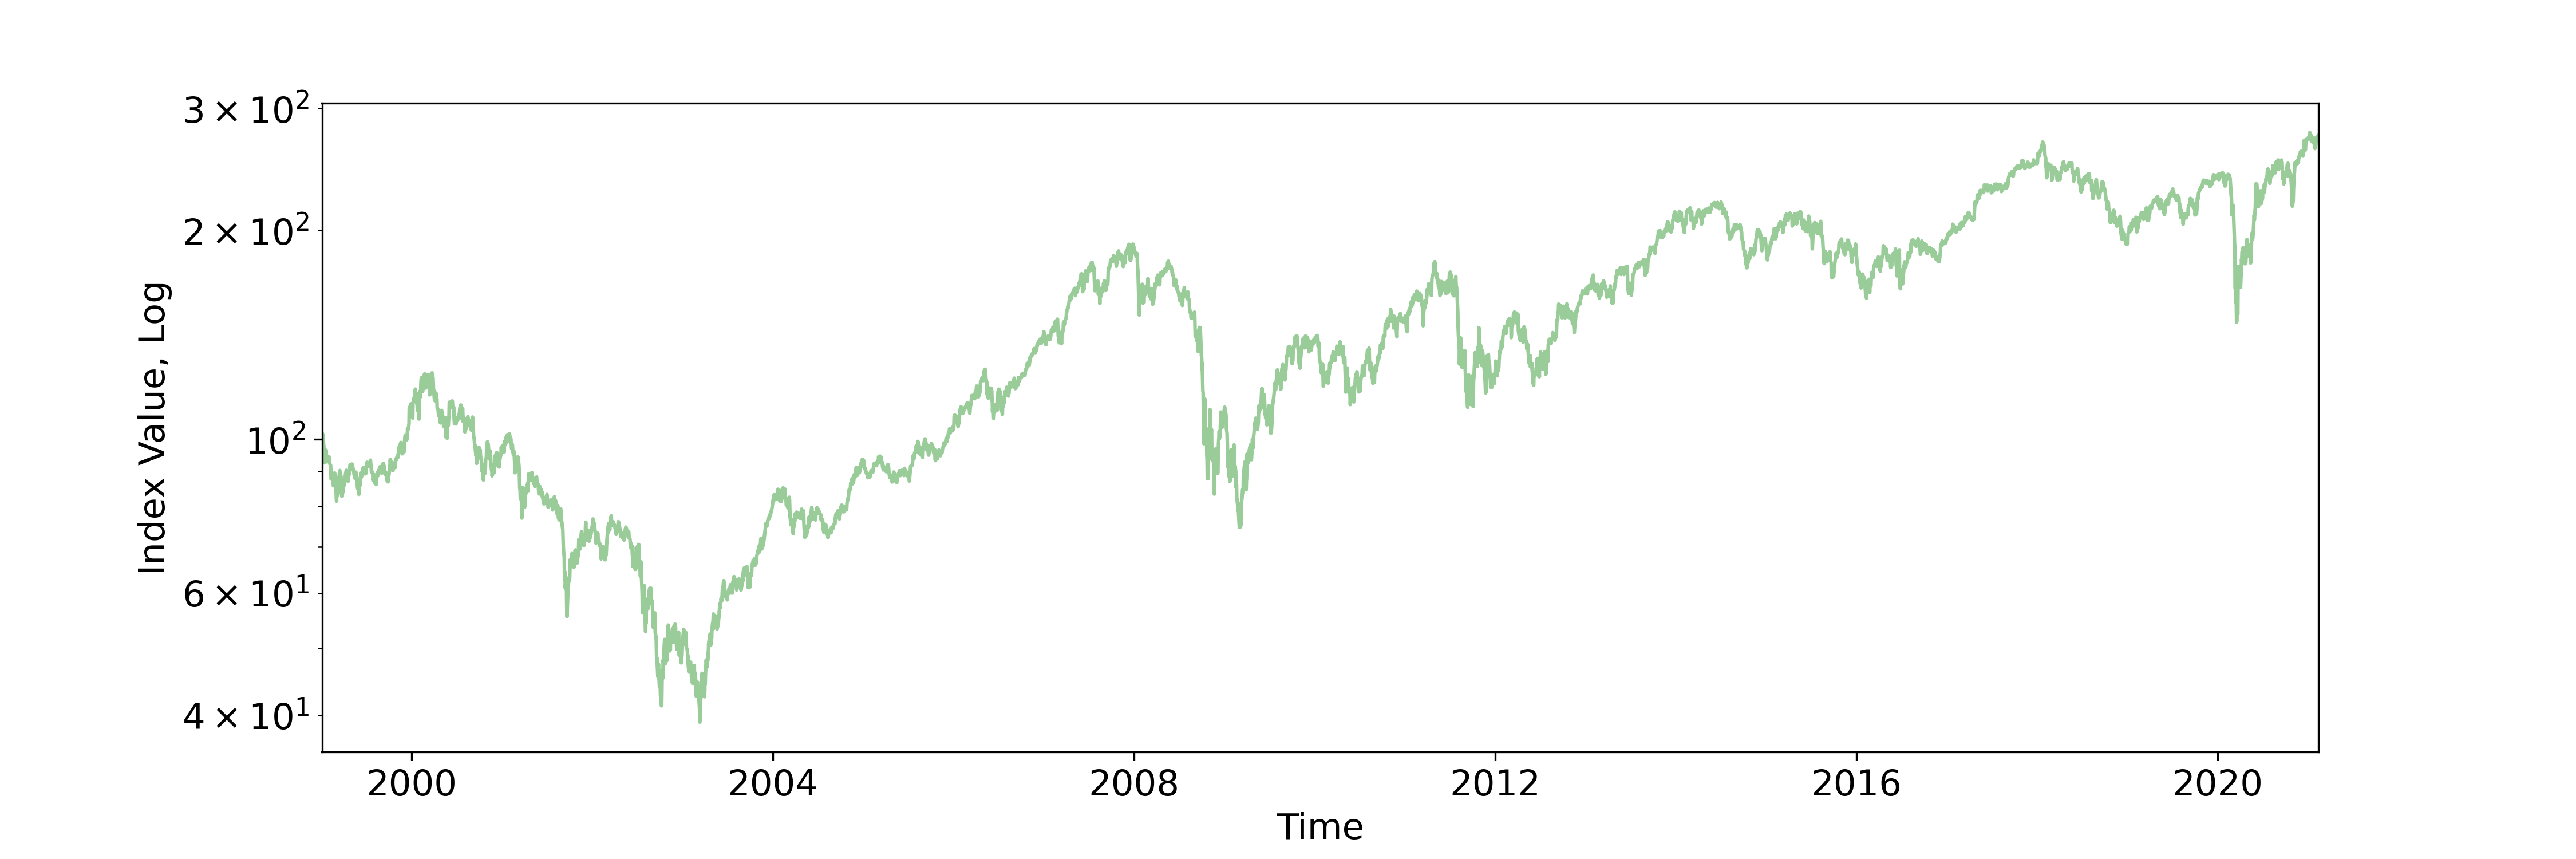
\includegraphics[width=1\textwidth]{analysis/data_description/images/DAX_index.png}
    \caption{Development DAX 30.}
    \label{fig: DAX_index}
\end{figure}

As is evident by figure \ref{fig: DAX_index}, the availability of daily data is significantly shorter compared to the MSCI World and the S\&P 500 Index. This is primarily due to the fact that the DAX 30 was originated in the late 1987. However, figure \ref{fig: DAX_index} also showcases that recent financial bear markets such as the dot-com bubble of the early 2000s, the GFC of 2008 as well as the COVID-19 rebound in Q1/Q2 2020 are well captured by DAX 30 Index. 

Since January 2006, the index is refreshed every second, however, the thesis will continue to rely on daily data frequencies as discussed in section \ref{subsection: Data frequency}. The index is capitalization-weighted and holds a total market capitalization of 1,017.7 billion EUR as of 21st of September 2020. In response to the recent accounting scandal related to Wirecard, Deutshce Börse announced an expansion of the DAX 30 to include 40 members. The expansion is set to occur in the third quarter of 2021.

\begin{table}[H]
\caption{Summary statistics for the daily DAX log-returns.}
\centering
\begin{tabular}{c c c c c c c c c} 
\hline\hline
Observations & Mean & STD & Skewness & Excess Kurtosis & Min & Max & First ACF & Annual SR \\
\hline
5,613 & 0.0002 & 0.0159 & -0.1869 & 2.8115 & -0.1394 & 0.1257 & 0.0146 & 0.1839 \\
\hline
\end{tabular}
\label{tab:summary_stats_DAX}
\end{table}

As highlighted by table \ref{tab:summary_stats_DAX}, the DAX Index contains much fewer observations compared to the MSCI World and S\&P 500 index. Furthermore, the DAX has similar mean daily returns although the standard deviation is the highest among the selected indices. However, the DAX is less negatively skewed and exhibit the lowest degree of leptokurtotic among the selected indexes. However, the high standard deviation naturally leads to a much lower Sharpe Ratio compared to the other indices at 0.1839.


##### Disitrbutional properties section:

The MSCI World Index appears to have a more stable trajectory with less volatile movements both compared to the S\&P 500 and the DAX 30. Despite this, the MSCI World Index generally trended in the same direction as the S\&P 500,
but in some periods the range between the two indices widened. For example,
it appears that the MSCI World and S\&P 500 Index trended in close correlation in the period from 1999 to 2015, however, from 2015 to 2021 the two indices have drifted apart. Furthermore, it appears that the S\&P 500 has become increasingly more volatile over the period 2015-2021, particularly evident by the recent COVID-19 rebound in which the drawdown of the S\&P 500 was much more extreme compared to the MSCI World.  

The DAX 30 performed particularly well in the period following the dot-com bubble, however, during 2008 and 2009 the GFC severely impacted the index, thereby bringing it down to the respective levels of the S\&P 500 and MSCI World. As concluded in section \ref{subsection: DAX 30} the DAX was characterised as the most volatile, which is also evident by figure \ref{fig: all_indices_index} which showcases that the DAX indeed appears to have a higher volatility. From 2006 to 2017 the DAX Index has consistently been at higher index levels compared to the other indices until the S\&P 500 caught up by breaking its all time high in 2019. An overview of the summary statistics for each index is listed in table \ref{tab:summary_all}.

#### LAst comment temporal properties

Conclusively, the reader should note that the correlation among the indices are stronger at the times of high market volatility. This is perhaps not surprising since the indices are made up of stocks, however, it highlights that diversification based on investing in different sectors or geographical areas may not materialize precisely when an investor needs it the most. The impact would most probably be less significant if one were to compare a stock index with a bond index, since the correlation would be lower, especially during periods of high volatility. Despite the fact that correlations increased in high volatility markets, there are definitely benefits related to diversification between asset classes.